\title{Problème de Syracuse}
\author{Arthur Jacquin}
\documentclass{hibiscus}

\usepackage{circuitikz}
\usepackage{pgfplots}
\pgfplotsset{width=10cm,compat=1.9}

\begin{document}
\maketitle
\tableofcontents

\section{Introduction}

\begin{equation*}
\begin{aligned}
f: \: \mathbb{N}^* & \longrightarrow \mathbb{N}^* \\
        n & \longmapsto \begin{cases} \frac{n}{2} & \text{ si } n \equiv 0 [2]
        \\ 3n + 1 & \text{ si } n \equiv 1 [2] \end{cases}
\end{aligned}
\end{equation*}

\par Voici la conjecture (non démontrée) de Syracuse : pour tout entier naturel $n$ non nul, l'ensemble $\left\{ k \in \mathbb{N} \: | \: f^k(n) = 1 \right\}$ est non vide donc admet un minimum. On cherche ici une façon efficace de vérifier ce résultat pour un $n$ donné (cela a déjà été fait jusqu'à $2^{68}$).

\par En supposant la conjecture vraie, on définit $m$ telle que :
\begin{equation*}
\begin{aligned}
m: \: \mathbb{N}^* & \longrightarrow \mathbb{N} \\
        n & \longmapsto \min \left\{ k \in \mathbb{N} \: | \: f^k(n) = 1 \right\}
\end{aligned}
\end{equation*}

\newpage \section{Circuits logiques - additions}

\subsection{Additionneur $1$ bit}

\par Le bloc \code{ADD} est défini par le circuit suivant. En binaire, on vérifie aisément que $a_1 + a_2 = b_2b_1$.

\begin{figure}[h!]
\begin{center}
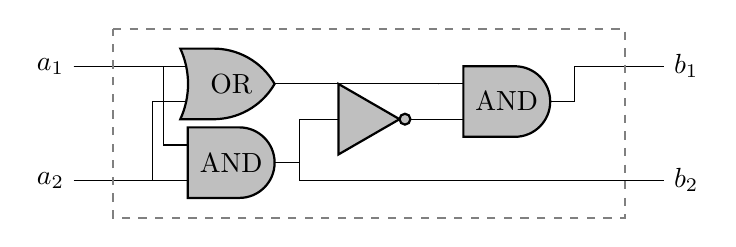
\begin{tikzpicture}
% Circuit style
\ctikzset{
    logic ports=ieee,
    logic ports/scale=0.8,
    logic ports/fill=lightgray
}

% Nodes
\node[left] (IN1) at (0, 0.724) {$a_1$};
\node[left] (IN2) at (0, -0.724) {$a_2$};
\node[below] (A) at (1, -0.724) {};

\node[or port] (OR) at (2, 0.5) {OR};
\node[and port] (ANDa) at (2, -0.5) {AND};
\node[not port] (NOT) at (3.75, 0.052) {};
\node[and port] (ANDb) at (5.5, 0.276) {AND};

\node[right] (OUT1) at (7.5, 0.724) {$b_1$};
\node[right] (OUT2) at (7.5, -0.724) {$b_2$};
 
% Connections
\draw (IN1) -| (OR.in 1);
\draw (IN1) -| (ANDa.in 1);
\draw (A) |- (OR.in 2);
\draw (IN2) -| (ANDa.in 2);

\draw (OR.out) -| (ANDb.in 1);
\draw (ANDa.out) |- (NOT.in);
\draw (NOT.out) -| (ANDb.in 2);

\draw (ANDb.out) |- (OUT1);
\draw (ANDa.out) |- (OUT2);

% Frame
\draw[thick, dashed, gray] (0.5, 1.2) -- ++(6.5, 0) -- ++(0, -2.4) -- ++(-6.5, 0) -- ++(0, 2.4);
\end{tikzpicture}
\caption{Bloc \code{ADD}.}
\end{center}
\end{figure}

\par On définit le bloc \code{ADDr} pour prendre en compte une éventuelle retenue. On a $r + a_1 + a_2 = b_2b_1$.

\begin{figure}[h!]
\begin{center}
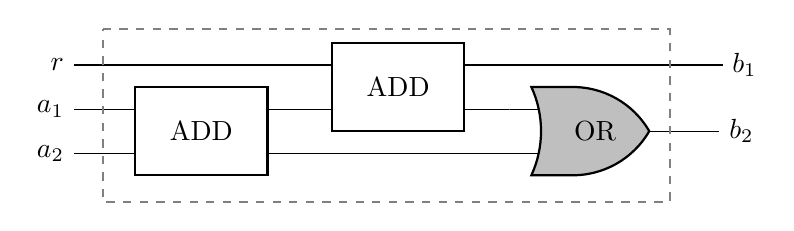
\begin{tikzpicture}
% Circuit style
\ctikzset{
    logic ports=ieee,
    logic ports/scale=1,
    logic ports/fill=lightgray
}

% Nodes
\node[dipchip, num pins=4, hide numbers, no topmark]
    (ADD1) at (0, 0) {ADD};
\node[dipchip, num pins=4, hide numbers, no topmark]
    (ADD2) at (2.5, 0.56) {ADD};
\node[or port] (OR) at (5, 0) {OR};

% Connections
\draw (ADD2.pin 1) -- ++(-3, 0) node[left] (IN1) {$r$};
\draw (ADD1.pin 1) -- ++(-0.5, 0) node[left] (IN2) {$a_1$};
\draw (ADD1.pin 2) -- ++(-0.5, 0) node[left] (IN3) {$a_2$};

\draw (ADD1.pin 4) -| (ADD2.pin 2);
\draw (ADD2.pin 3) -| (OR.in 1);
\draw (ADD1.pin 3) -| (OR.in 2);

\draw (ADD2.pin 4) -- ++(3, 0) node[right] (OUT1) {$b_1$};
\draw (OR.out) -- ++(0.5, 0) node[right] (OUT2) {$b_2$};
 
% Frame
\draw[thick, dashed, gray] (-1.25, 1.3) -- ++(7.2, 0) -- ++(0, -2.2) -- ++(-7.2, 0) -- ++(0, 2.2);
\end{tikzpicture}
\caption{Bloc \code{ADDr}.}
\end{center}
\end{figure}

\subsection{Additionneur $n$ bits}

\par Le circuit suivant est un additionneur $4$ bits et donne $a_4a_3a_2a_1 + b_4b_3b_2b_1 = c_5c_4c_3c_2c_1$. La généralisation à $n$ bits est immédiate.

\begin{figure}[h!]
\begin{center}
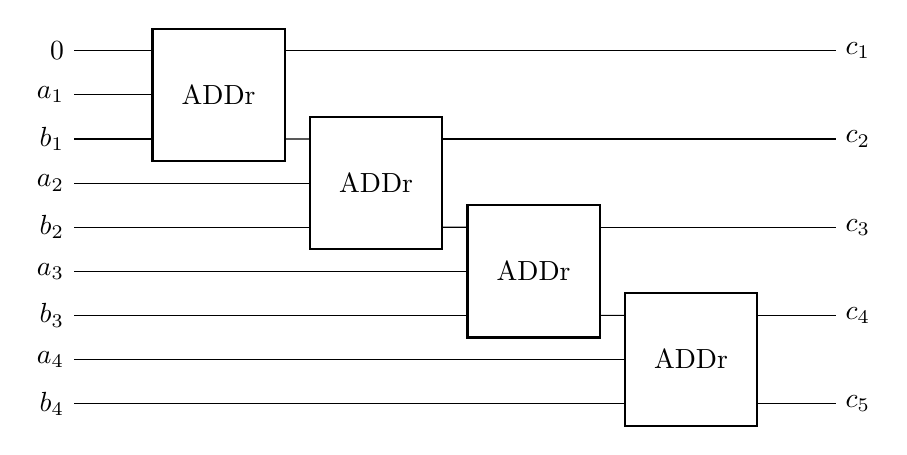
\begin{tikzpicture}
% Circuit style
\ctikzset{
    logic ports=ieee,
    logic ports/scale=1,
    logic ports/fill=lightgray
}

% Nodes
\node[dipchip, num pins=6, hide numbers, no topmark, external pins width=0] (AR1) at (0, 0) {ADDr};
\node[dipchip, num pins=6, hide numbers, no topmark, external pins width=0] (AR2) at (2, -1.12) {ADDr};
\node[dipchip, num pins=6, hide numbers, no topmark, external pins width=0] (AR3) at (4, -2.24) {ADDr};
\node[dipchip, num pins=6, hide numbers, no topmark, external pins width=0] (AR4) at (6, -3.36) {ADDr};
 
% Connections
\draw (AR1.pin 1) -- ++(-1, 0) node[left] (IN0) {$0$};

\draw (AR1.pin 2) -- ++(-1, 0) node[left] (IN1) {$a_1$};
\draw (AR1.pin 3) -- ++(-1, 0) node[left] (IN2) {$b_1$};
\draw (AR1.pin 6) -- ++(7, 0) node[right] (OUT1) {$c_1$};
\draw (AR1.pin 4) -- (AR2.pin 1);

\draw (AR2.pin 2) -- ++(-3, 0) node[left] (IN3) {$a_2$};
\draw (AR2.pin 3) -- ++(-3, 0) node[left] (IN4) {$b_2$};
\draw (AR2.pin 6) -- ++(5, 0) node[right] (OUT2) {$c_2$};
\draw (AR2.pin 4) -- (AR3.pin 1);

\draw (AR3.pin 2) -- ++(-5, 0) node[left] (IN5) {$a_3$};
\draw (AR3.pin 3) -- ++(-5, 0) node[left] (IN6) {$b_3$};
\draw (AR3.pin 6) -- ++(3, 0) node[right] (OUT3) {$c_3$};
\draw (AR3.pin 4) -- (AR4.pin 1);

\draw (AR4.pin 2) -- ++(-7, 0) node[left] (IN7) {$a_4$};
\draw (AR4.pin 3) -- ++(-7, 0) node[left] (IN8) {$b_4$};
\draw (AR4.pin 6) -- ++(1, 0) node[right] (OUT4) {$c_4$};
\draw (AR4.pin 4) -- ++(1, 0) node[right] (OUT5) {$c_5$};
\end{tikzpicture}
\caption{Additionneur $4$ bits.}
\end{center}
\end{figure}


\newpage \section{Application au problème de Syracuse}

\begin{description}
\item[Objectif] Itérer efficacement dans l'algorithme de Syracuse.
\end{description}

\par Soit $n = \sum_{i=0}^{l}{a_i 2^i} \in \mathbb{N}$. Le cas $n$ pair n'est pas très intéressant : la prochaine itération ($f(n) = \frac{n}{2}$) correspond à un simple décalage des bits. Essayons donc d'implémenter l'itération pour $n$ impair ($f(n) = 3n + 1$). On remarque que $f(n)$ est alors pair : on peut donc itérer deux fois en obtenant directement $f^2(n) = \frac{3n+1}{2}$.

\medskip \par On remarque que $3n+1 = (n) + (2n+1)$. Ces deux quantités sont très faciles à former : $n$ est déjà formé, $2n+1$ est (en binaire) la concaténation des bits de $n$ et de $1$. On traitera l'addition restante par le même méchanisme qu'en partie 1, ici en supposant $l = 2$.

\begin{figure}[h!]
\begin{center}
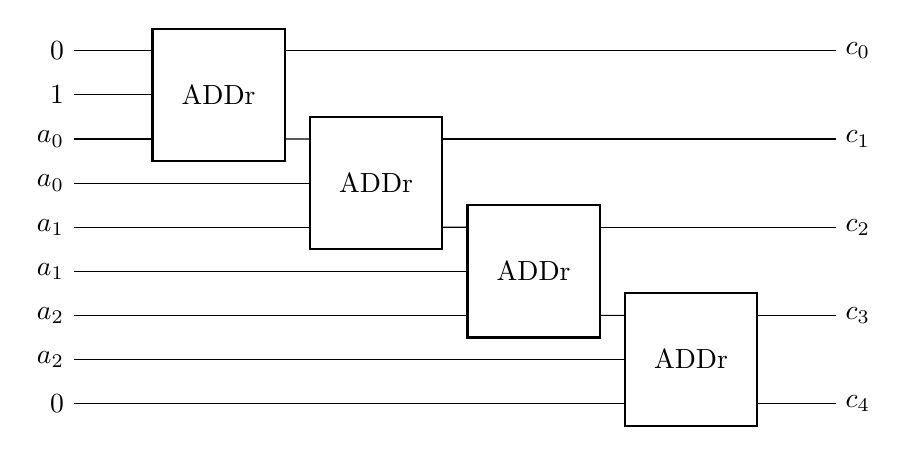
\begin{tikzpicture}
% Circuit style
\ctikzset{
    logic ports=ieee,
    logic ports/scale=1,
    logic ports/fill=lightgray
}

% Nodes
\node[dipchip, num pins=6, hide numbers, no topmark, external pins width=0] (AR1) at (0, 0) {ADDr};
\node[dipchip, num pins=6, hide numbers, no topmark, external pins width=0] (AR2) at (2, -1.12) {ADDr};
\node[dipchip, num pins=6, hide numbers, no topmark, external pins width=0] (AR3) at (4, -2.24) {ADDr};
\node[dipchip, num pins=6, hide numbers, no topmark, external pins width=0] (AR4) at (6, -3.36) {ADDr};
 
% Connections
\draw (AR1.pin 1) -- ++(-1, 0) node[left] (IN0) {$0$};

\draw (AR1.pin 2) -- ++(-1, 0) node[left] (IN1) {$1$};
\draw (AR1.pin 3) -- ++(-1, 0) node[left] (IN2) {$a_0$};
\draw (AR1.pin 6) -- ++(7, 0) node[right] (OUT1) {$c_0$};
\draw (AR1.pin 4) -- (AR2.pin 1);

\draw (AR2.pin 2) -- ++(-3, 0) node[left] (IN3) {$a_0$};
\draw (AR2.pin 3) -- ++(-3, 0) node[left] (IN4) {$a_1$};
\draw (AR2.pin 6) -- ++(5, 0) node[right] (OUT2) {$c_1$};
\draw (AR2.pin 4) -- (AR3.pin 1);

\draw (AR3.pin 2) -- ++(-5, 0) node[left] (IN5) {$a_1$};
\draw (AR3.pin 3) -- ++(-5, 0) node[left] (IN6) {$a_2$};
\draw (AR3.pin 6) -- ++(3, 0) node[right] (OUT3) {$c_2$};
\draw (AR3.pin 4) -- (AR4.pin 1);

\draw (AR4.pin 2) -- ++(-7, 0) node[left] (IN7) {$a_2$};
\draw (AR4.pin 3) -- ++(-7, 0) node[left] (IN8) {$0$};
\draw (AR4.pin 6) -- ++(1, 0) node[right] (OUT4) {$c_3$};
\draw (AR4.pin 4) -- ++(1, 0) node[right] (OUT5) {$c_4$};
\end{tikzpicture}
\caption{Itérateur $n = \sum{a_i2^i} \longmapsto 3n+1 = \sum{c_i2^i}$ pour $l = 2$.}
\end{center}
\end{figure}

\par On admet que $n$ est impair, c'est-à-dire que $a_0 = 1$. Enfin, comme $3n+1$ est pair, $c_0 = 0$. Ces deux informations étant connues, on peut simplifier le circuit. Ignorer $c_0$ permet également de diviser par $2$. La généralisation à un $l$ quelconque est immédiate.

\begin{figure}[h!]
\begin{center}
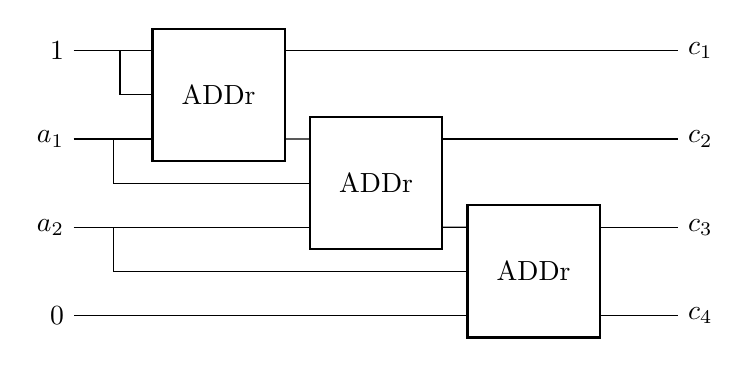
\begin{tikzpicture}
% Circuit style
\ctikzset{
    logic ports=ieee,
    logic ports/scale=1,
    logic ports/fill=lightgray
}

% Nodes
\node[dipchip, num pins=6, hide numbers, no topmark, external pins width=0] (AR1) at (0, 0) {ADDr};
\node[dipchip, num pins=6, hide numbers, no topmark, external pins width=0] (AR2) at (2, -1.12) {ADDr};
\node[dipchip, num pins=6, hide numbers, no topmark, external pins width=0] (AR3) at (4, -2.24) {ADDr};
 
% Connections
\draw (AR1.pin 1) -- ++(-1, 0) node[left] (IN0) {$1$};

\draw (IN0) -- ++(0.8, 0) |- (AR1.pin 2);
\draw (AR1.pin 3) -- ++(-1, 0) node[left] (IN1) {$a_1$};
\draw (AR1.pin 6) -- ++(5, 0) node[right] (OUT1) {$c_1$};
\draw (AR1.pin 4) -- (AR2.pin 1);

\draw (IN1) -- ++(0.8, 0) |- (AR2.pin 2);
\draw (AR2.pin 3) -- ++(-3, 0) node[left] (IN2) {$a_2$};
\draw (AR2.pin 6) -- ++(3, 0) node[right] (OUT2) {$c_2$};
\draw (AR2.pin 4) -- (AR3.pin 1);

\draw (IN2) -- ++(0.8, 0) |- (AR3.pin 2);
\draw (AR3.pin 3) -- ++(-5, 0) node[left] (IN3) {$0$};
\draw (AR3.pin 6) -- ++(1, 0) node[right] (OUT3) {$c_3$};
\draw (AR3.pin 4) -- ++(1, 0) node[right] (OUT4) {$c_4$};
\end{tikzpicture}
\caption{Itérateur $n = \sum{a_i2^i} \longmapsto \frac{3n+1}{2} = \sum{c_i2^{i-1}}$ pour $l = 2$.}
\end{center}
\end{figure}

\newpage \section{Implémentation en Python}

\par On ne s'attache pas à l'optimisation de ce script ou à l'utilisation d'un fonctionnement fin de Python : ce n'est qu'une étape avant une implémentation en C, qui permettra de gérer finement les opérations sur les bits et ainsi de profiter du travail sur les circuits logiques. Par exemple, on ne soulèvera pas d'erreurs (ce méchanisme n'existe pas en C) mais nous renverrons une valeur associée à l'erreur.

\medskip \par Intéressons nous dans un premier temps aux nombres impairs (utilisation de la figure précédente). En ne formant $f(n)$ qu'à partir de la détection d'un $1$, on peut se ramener directement au nombre impair $\frac{f(n)}{2^{Val_2(f(n))}}$. En ne manipulant uniquement des nombres impairs, on peut omettre le premier bit (correspondant à la parité). Pour étendre les fonctions aux nombres pairs, il suffit de remarquer que $m(n) = Val_2(n) + m(\frac{n}{2^{Val_2(n)}})$.

\medskip \par Définissons un nombre de bit maximal pour la représentation des entiers : \code{l = 32}. L'omission des bits de signe et la division systématique par $2^{Val_2(n)}$ permet de manipuler des quantités bien supérieures à $2^l$. La fonction \code{iter_impair} considère donc une représentation binaire privée de son bit de parité d'un impair $n$ et renvoie :
\begin{itemize}
\item La représentation binaire privée de son bit de parité de $n'$, résultat des multiples itérations effectuées.
\item Le nombre d'itérations effectuées par l'éxécution de la fonction. La fonction se base sur la figure précédente, qui opère déjà 2 itérations, mais chaque zéro ignoré avant d'écrire $n'$ correspond également à une itération. 
\item Le nombre de bits significatifs de $n'$. S'il est nul, cela signifie que $n' = 2*0 + 1$, donc que l'on a opéré $m(n)$ itérations. S'il est strictement supérieur à $l$, il y a dépassement de capacité de stockage (\textit{overflow}) : il est nécessaire d'augmenter $l$ pour traiter $n$.
\end{itemize}

\medskip \par Enfin, on étends l'utilisation de la fonction à $\mathbb{N}^*$ avec la fonction \code{m}. Le script de la page suivante permet d'obtenir les résultats suivants :

\begin{figure}[h!]
\begin{center}
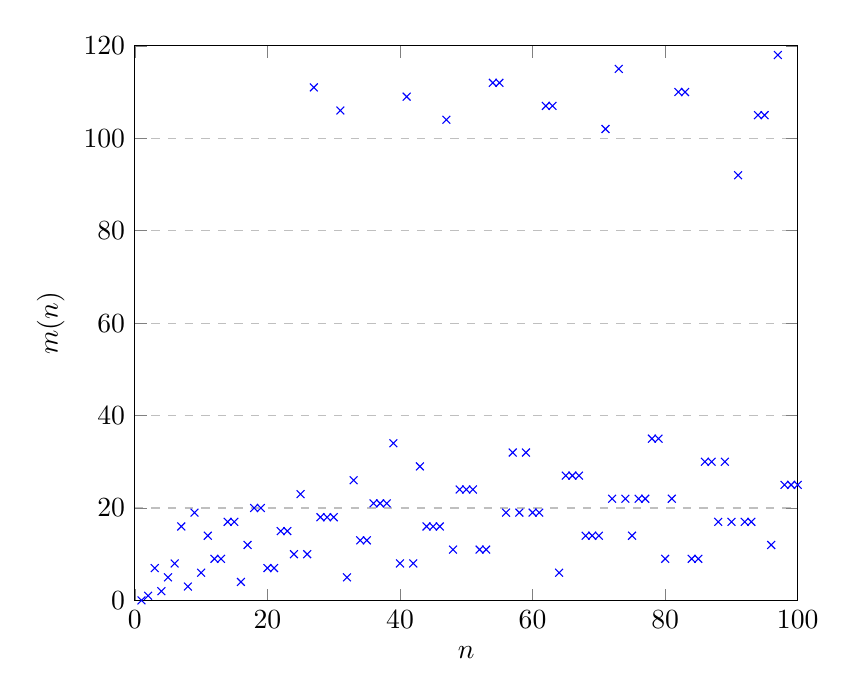
\begin{tikzpicture}
\begin{axis}[
    xlabel={$n$},
    ylabel={$m(n)$},
    xmin=0, xmax=100,
    ymin=0, ymax=120,
    xtick={0,20,40,60,80,100},
    ytick={0,20,40,60,80,100,120},
    legend pos=north west,
    ymajorgrids=true,
    grid style=dashed,
]

\addplot[only marks, blue, mark=x] coordinates {
    (1,0)(2,1)(3,7)(4,2)(5,5)(6,8)(7,16)(8,3)(9,19)(10,6)
    (11,14)(12,9)(13,9)(14,17)(15,17)(16,4)(17,12)(18,20)(19,20)(20,7)
    (21,7)(22,15)(23,15)(24,10)(25,23)(26,10)(27,111)(28,18)(29,18)(30,18)
    (31,106)(32,5)(33,26)(34,13)(35,13)(36,21)(37,21)(38,21)(39,34)(40,8)
    (41,109)(42,8)(43,29)(44,16)(45,16)(46,16)(47,104)(48,11)(49,24)(50,24)
    (51,24)(52,11)(53,11)(54,112)(55,112)(56,19)(57,32)(58,19)(59,32)(60,19)
    (61,19)(62,107)(63,107)(64,6)(65,27)(66,27)(67,27)(68,14)(69,14)(70,14)
    (71,102)(72,22)(73,115)(74,22)(75,14)(76,22)(77,22)(78,35)(79,35)(80,9)
    (81,22)(82,110)(83,110)(84,9)(85,9)(86,30)(87,30)(88,17)(89,30)(90,17)
    (91,92)(92,17)(93,17)(94,105)(95,105)(96,12)(97,118)(98,25)(99,25)(100,25)};
\end{axis}
\end{tikzpicture}
\caption{$n \longmapsto m(n)$.}
\end{center}
\end{figure}

\newpage \lstinputlisting[caption=\code{syracuse.py}, language=Python]{syracuse.py}

\newpage \section{Implémentation en C}

\lstinputlisting[caption=\code{syracuse.c}, language=C]{syracuse.c}

\newpage \section{Comparaison des performances}

\begin{tabular}{p{0.45\textwidth} p{0.45\textwidth}}
\lstinputlisting[caption=\code{syracuse_naif.py}, language=Python]{syracuse_naif.py}
&
\lstinputlisting[caption=\code{syracuse_naif.c}, language=Caml]{syracuse_naif.c}
\end{tabular}

\par On mesure le temps de calcul des $m(n)$ avec $n \in \lentint 1; N \rentint$. Les versions en C sont (à méthode identique) notablement plus rapides, probablement grâce à la compilation. En revanche, les versions naïves sont (à language identique) notablement plus rapides : les efforts d'optimisations ont été inutiles.

\begin{figure}[h!]
\begin{center}
\begin{tikzpicture}
\begin{loglogaxis}[
    xlabel={Nombre $N$ de valeurs calculées},
    ylabel={Temps de calcul (s)},
    ymin=0.01, ymax=1000,
    ytick={0.1, 1, 10, 100},
    legend pos=north west,
    ymajorgrids=true,
    grid style=dashed,
]

\addplot[blue, mark=*] plot coordinates {
    (1000,0.09)(10000,0.36)(100000,4.04)(1000000,45.37)};
\addlegendentry{\code{syracuse_naif.py}}

\addplot[green, mark=*] plot coordinates {
    (1000,14.56)(10000,199.37)};
\addlegendentry{\code{syracuse.py}}

\addplot[mark=*] plot coordinates {
    (1000,0.01)(10000,0.01)(100000,0.1)(1000000,1.15)};
\addlegendentry{\code{syracuse_naif.c}}

\addplot[red, mark=*] plot coordinates {
    (1000,0.03)(10000,0.45)(100000,5.36)(1000000,64.82)};
\addlegendentry{\code{syracuse.c}}
\end{loglogaxis}
\end{tikzpicture}
\caption{Comparaison des scripts}
\end{center}
\end{figure}
\end{document}
